\documentclass{beamer}
\usetheme{metropolis} % Use metropolis theme
\usepackage{lmodern}

\renewcommand{\footnoterule}{%
  \hspace{2cm}
  \kern -3pt
  \hrule width \textwidth height 1pt
  \kern 2pt
}
\usepackage[utf8]{inputenc}
\usepackage[T1]{fontenc}
\usepackage[autostyle, english = british]{csquotes}
\usepackage[british]{babel}
\usepackage{todonotes}
\usepackage[%
  backend=biber,
  doi=false,
  url=false,
  isbn=false,
  eprint=false,
  style=verbose,
  citestyle=verbose,
  hyperref=true,
  maxnames=99,
  minnames=1,
  maxbibnames=99,
  firstinits,
  uniquename=init]{biblatex}
%\DeclareFieldFormat[inproceedings, article]{pages}{}%
%\DeclareFieldFormat[inproceedings]{organization}{}%
  % ignore some field for citations
\DeclareSourcemap{
  \maps[datatype=bibtex, overwrite]{
    \map{
      \step[fieldset=edition, null]
      \step[fieldset=publisher, null]
      \step[fieldset=pages, null]
      \step[fieldset=organization, null]
    }
  }
}

\addbibresource{../bibliography.bib}

\let\oldfootnotesize\footnotesize
\renewcommand*{\footnotesize}{\oldfootnotesize\fontsize{6}{6}}

\usepackage{caption}
\usepackage{xpatch}
\usepackage{bm}
\usepackage{amsmath}
\usepackage{mathtools} % for \mathclap
\usepackage{varioref}
\usepackage{siunitx}
\usepackage{hyperref}
\usepackage[noabbrev]{cleveref}
\newcommand{\creflastconjunction}{, and\nobreakspace} % use Oxford comma
\usepackage{todonotes}
\usepackage{multimedia}
\usepackage{tikz}
\usetikzlibrary{arrows, positioning, shapes.geometric}
\usetikzlibrary{calc}
\usepackage{pgfgantt}


\graphicspath{{../../figures/}}

\newcommand{\cn}{\footnote{\enquote{TODO: Citation.}, 2017, \textbf{Conference}, \textit{Author 1, Author 2, Author 3, Author 4} }}

\title{Deep-Learning-based Image Denoising in Ophthalmology\\Guided Research Kick-Off}
\author{Lukas Krenz\\Adviser: Nicola Rieke\\Director: Prof.\ Dr.\ Nassir Navab}
\date{January 19, 2018} 
\institute{TUM, Chair for Computer Aided Medical Procedures \textit{\&} Augmented Reality}

\begin{document}
\maketitle

\begin{frame}
  \frametitle{Example Use-Case: Digital Window}
   \begin{figure}[h]
    \centering
    \movie[width=0.9735\textwidth, height=0.55\textwidth, autostart,, loop, poster]{}{digitalwindow.mp4}
    \caption*{Digital Window}
    \label{fig:digital-window}
  \end{figure}
\end{frame}


\begin{frame}{What are we trying to do?}
\begin{block}{Idea}
\begin{itemize}
\item Improve quality of retinal images by super-resolution \textit{\&} deblurring
\item Should work in an intraoperative setting
\end{itemize}
\end{block}

\begin{block}{Use cases}
\begin{itemize}
\item Pre-processing for other computer vision algorithms
\item Provide improved quality for digital zoom
\end{itemize}
\end{block}

\begin{block}{Constraints}
  \begin{itemize}
  \item Real-time, as fast as possible
  \item Different levels of zoom
  \item Preserve anatomical structure (vessels, etc.)
  \end{itemize}
\end{block}
\end{frame}

\begin{frame}
  \frametitle{State of the Art}

\begin{block}{General Super-Resolution}
Many different super resolution approaches\footcite{SRsurvey}.
    
E.g.\ based on image statistics, self-similarity of images, learned patch-databases or \textbf{convolutional neural networks}

CNNs fulfil \textbf{both} quality and speed constraints
\end{block}


\begin{block}{Ophthalmology}
Uses CNN-Upscaling\footcite{SaliencyGAN} 

Solid results, not optimised for intraoperative use-case
\end{block}
\end{frame}

\begin{frame}{Some common CNN-Topologies\footcite{LapSRN}}
\begin{columns}
\begin{column}{0.33\textwidth}
  \begin{figure}[h]
    \centering
    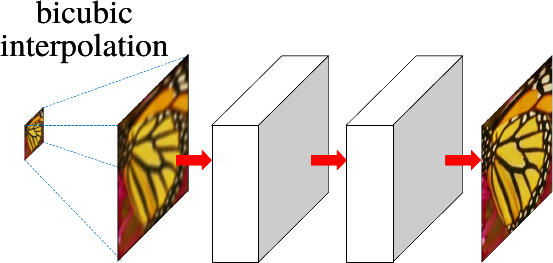
\includegraphics[height=0.4\textwidth]{sr_architectures_srcnn}
    \caption*{SRCNN\footnotemark}
  \end{figure}
\end{column} \footcitetext{Srcnn}\begin{column}{0.33\textwidth}
  \begin{figure}[h]
    \centering
    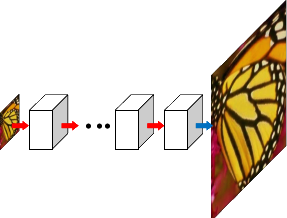
\includegraphics[height=0.4\textwidth]{sr_architectures_fsrcnn}
    \caption*{FSRCNN\footnotemark}
  \end{figure}
\end{column}
\footcitetext{Fsrcnn}
\end{columns}

\begin{columns}
\begin{column}{0.66\textwidth}
  \begin{figure}[h]
    \centering
    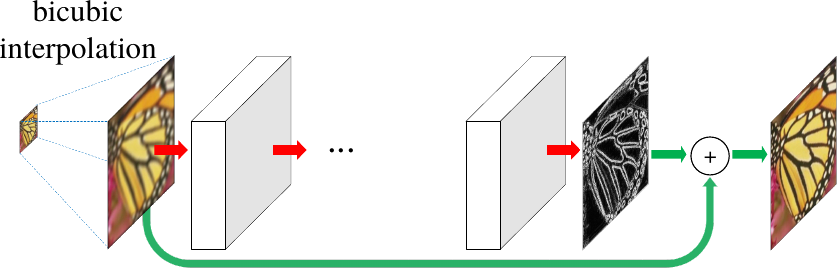
\includegraphics[width=0.6\textwidth]{sr_architectures_vdsr}
    \caption*{VDSR\footnotemark}
  \end{figure}
\end{column}
\footcitetext{Vdsr}
\begin{column}{0.34\textwidth}
  \textit{Red}: Convolution\\
  \textit{Blue}: Transposed Convolution\\
  \textit{Green}: Summation
\end{column}
\end{columns}
\end{frame}

\begin{frame}{Laplacian Network\footfullcite{LapSRN}}
\begin{columns}
\begin{column}{0.66\textwidth}
  \begin{figure}[h]
    \centering
    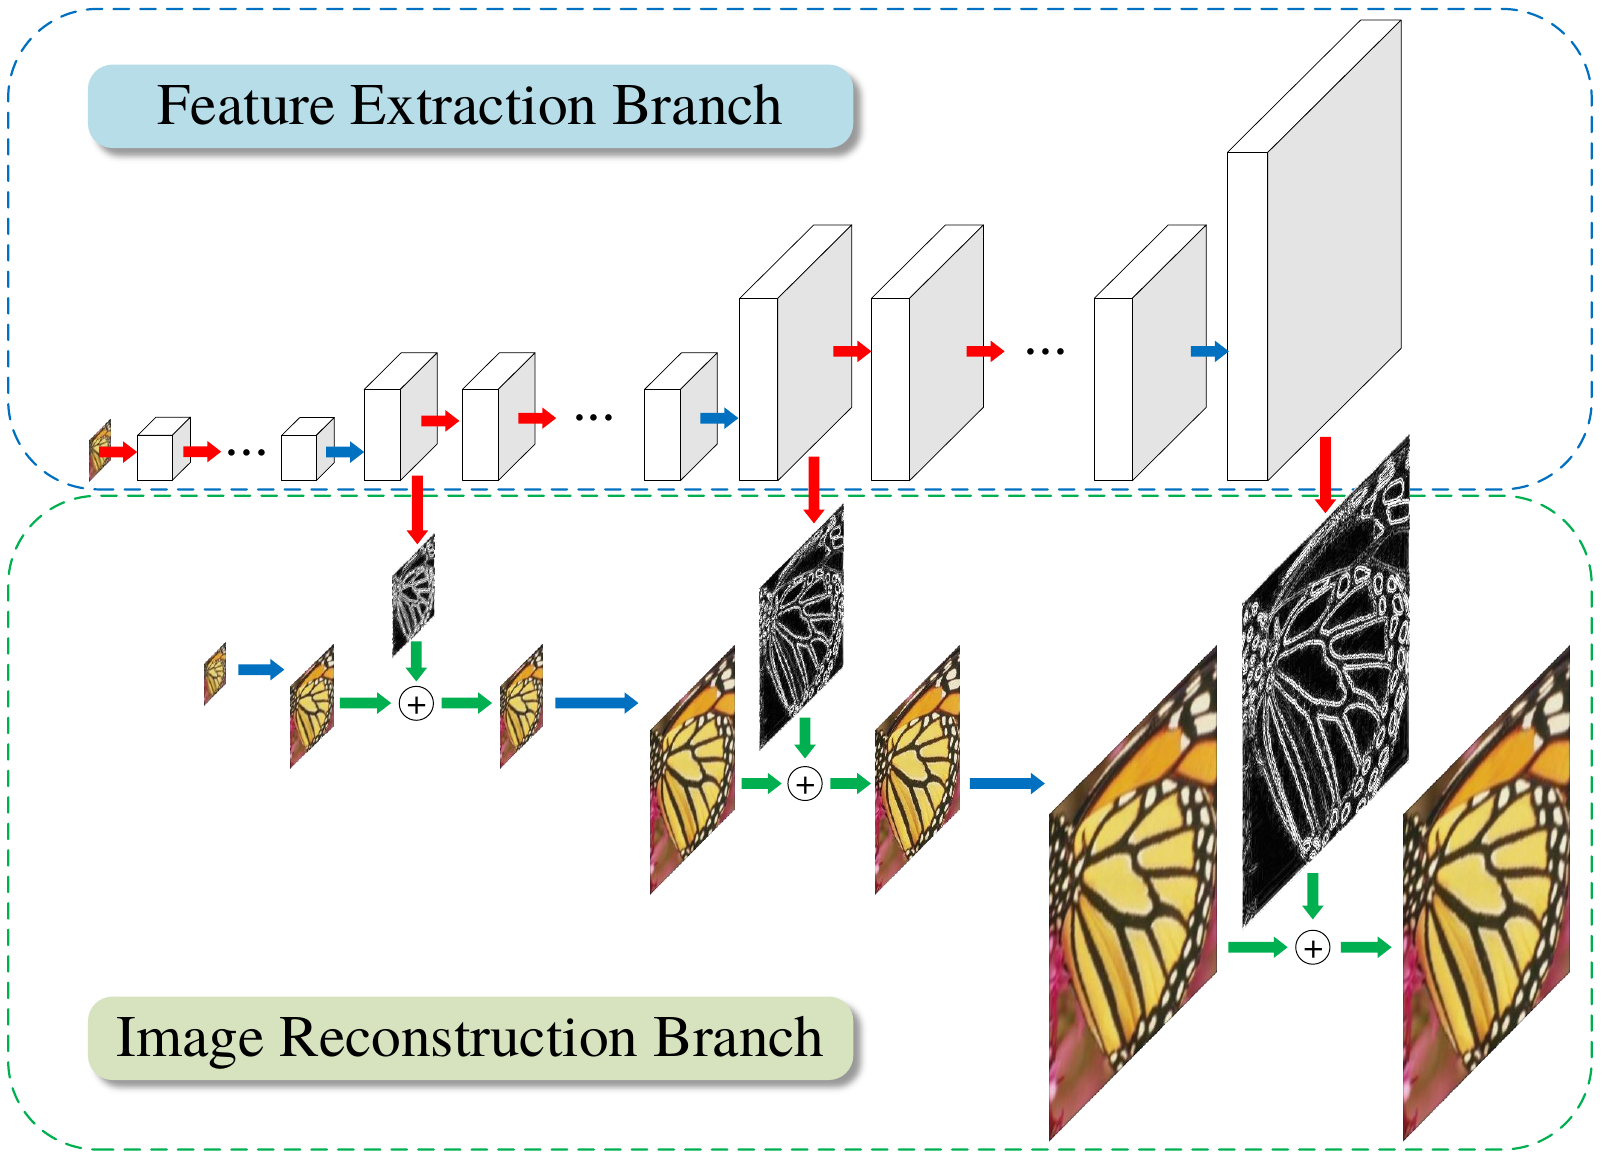
\includegraphics[width=1.0\textwidth]{lap_srn.png}
    \caption*{Laplacian pyramid network}
    \label{fig:lap-srn}
  \end{figure}
\end{column}

\begin{column}{0.34\textwidth}
  \begin{enumerate}
  \item Residual Learning
  \item Progressive Reconstruction
  \item Low-resolution filters
  \item Non-SR-case: Add residual to HR-images
  \end{enumerate}
\end{column}
\end{columns}
\textit{Red}: $3 \times 3$ convolution, \textit{blue}: transposed convolution, \textit{green} summation
\end{frame}

\begin{frame}{Robust (Charbonnier) Loss\footfullcite{LapSRN}}
(Relaxed) $L_1$  loss instead of $L_2$ loss
\begin{align*}
    \label{eq:charbonnier}
    L( \hat{\bm{y}}, \bm{y}; \bm{\theta}) &= \sum_n p \left( \bm{\hat{y}} - \bm{y} \right)\\
    %\shortintertext{with }
    p(\bm{x}) &= \sqrt{ \langle x, x \rangle  + \epsilon^2},
  \end{align*}

Robust, avoids \textbf{blurry} images

\begin{columns}
  \begin{column}{0.33\linewidth}
    \begin{figure}[h]
      \centering
        
\includegraphics[width=0.9\textwidth]{loss_functions_lap_l2}
      \caption*{$L_2$ loss}
    \end{figure}
  \end{column}
  \begin{column}{0.33\linewidth}
    \begin{figure}[h]
      \centering
        
\includegraphics[width=0.9\textwidth]{loss_functions_lap_l1}
      \caption*{$L_1$ loss}
    \end{figure}
  \end{column}  \begin{column}{0.33\linewidth}
    \begin{figure}[h]
      \centering
        
\includegraphics[width=0.9\textwidth]{loss_functions_lap_gt}
      \caption*{Ground truth}
    \end{figure}
  \end{column}
\end{columns}
\end{frame}

\begin{frame}{Perceptual Loss---VGG-based\footcite{PerceptualLoss}}
Transform images before calculating loss, with feature map $\phi$:
\begin{equation*}
    L_p( \hat{\bm{y}}, \bm{y}; \bm{\theta}) = \sum_n \Vert \phi( \bm{\hat{y}} ) - \phi( \bm{y}) \Vert
\end{equation*}

  \alert{Possibility 1}: Neural Network based loss, \textbf{automatic} features

  Extract feature maps from pre-trained VGG16-Network
\begin{columns}
  \begin{column}{0.33\linewidth}
    \begin{figure}[h]
      \centering
        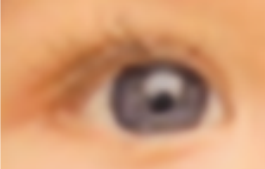
\includegraphics[width=0.9\textwidth]{perceptual_loss_l2}
      \caption*{$L_2$ loss}
    \end{figure}
  \end{column}
  \begin{column}{0.33\linewidth}
    \begin{figure}[h]
      \centering
        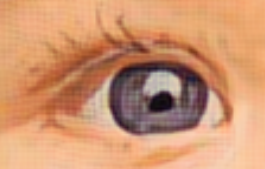
\includegraphics[width=0.9\textwidth]{perceptual_loss_vgg}
      \caption*{Perceptual loss}
    \end{figure}
  \end{column}  \begin{column}{0.33\linewidth}
    \begin{figure}[h]
      \centering
        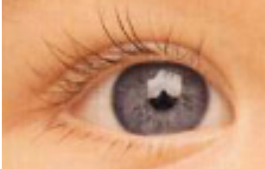
\includegraphics[width=0.9\textwidth]{perceptual_loss_gt}
      \caption*{Ground truth}
    \end{figure}
  \end{column}
\end{columns}
\end{frame}

\begin{frame}
  \frametitle{Perceptual Loss---Saliency Maps\footfullcite{SaliencyGAN}}
   \alert{Possibility 2}: Saliency Maps

  \textbf{Handcrafted} features
\begin{columns}
  \begin{column}{0.5\linewidth}
    \begin{figure}[h]
      \centering
        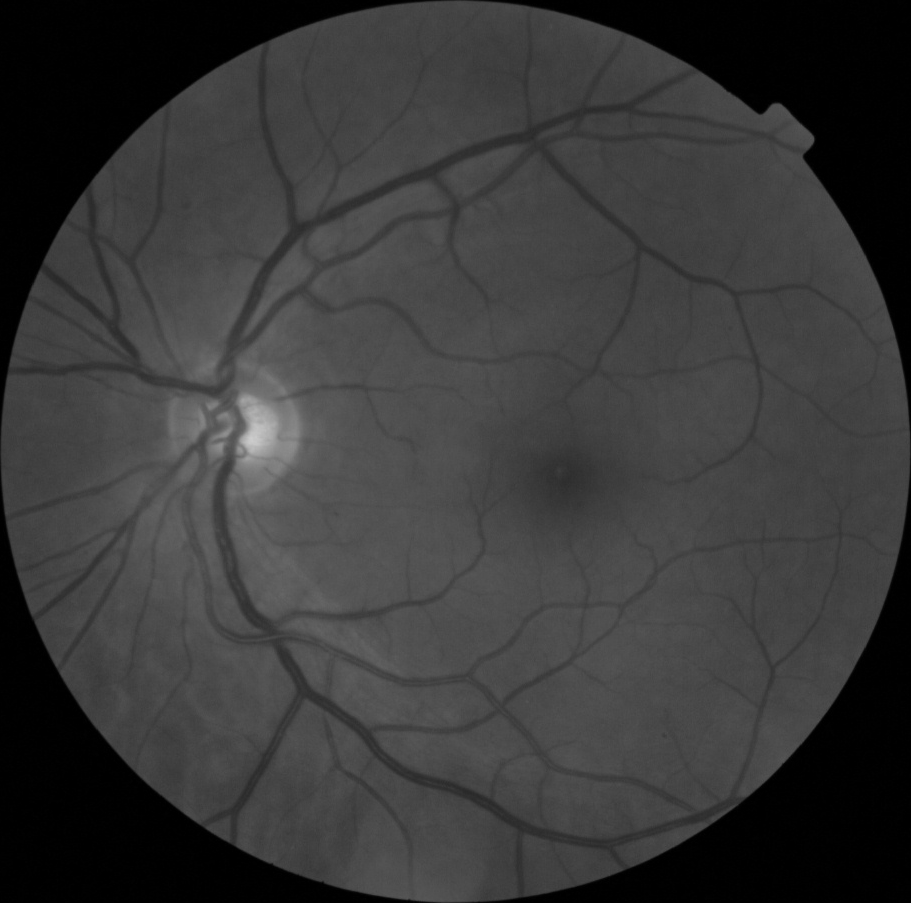
\includegraphics[width=0.9\textwidth]{saliency_gt}
      \caption*{Retina image}
    \end{figure}
  \end{column}
  \begin{column}{0.5\linewidth}
    \begin{figure}[h]
      \centering
        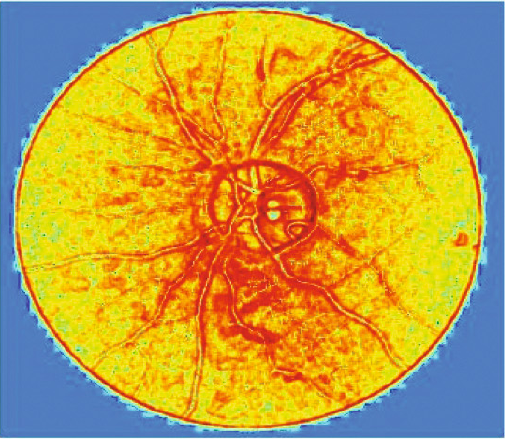
\includegraphics[width=0.9\textwidth]{saliency_smap}
      \caption*{Resulting saliency map}
    \end{figure}
  \end{column} 
\end{columns}
\end{frame}

\begin{frame}{Adversarial Loss}
  Two player game between
  \begin{description}
  \item[Generator] Super-resolution network
  \item[Discriminator] Tries to decide, whether images are \textbf{real} high-resolution images or \textbf{generated} by our network
  \end{description}

  Leads to realistic looking images
\begin{figure}[h]
    \centering
    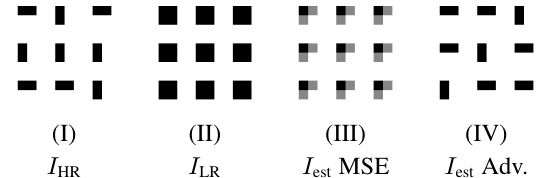
\includegraphics[width=0.58\textwidth]{adversarial_loss}
    \caption*{Toy example for adversarial loss\footcite{EnhanceNet}}
  \end{figure}
\end{frame}

\begin{frame}{Possible Modifications for Network}
  Weight sharing

  Replace stacked convolutions

  Replace transposed convolutions (avoid checkerboard artifacts)\footfullcite{deconvolution}

  \begin{figure}[h]
    \centering
    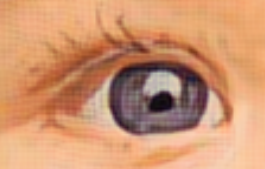
\includegraphics[width=0.45\textwidth]{perceptual_loss_vgg}
    \caption*{Example of block artifacts (from \footfullcite{PerceptualLoss})}
  \end{figure}
\end{frame}

\begin{frame}
   \frametitle{Dataset}
   Use 1000 images from Eyepacs dataset\footnote{\url{https://www.kaggle.com/c/diabetic-retinopathy-detection}} (ca.\ 30k HR) for training

   Augment, then select random crops of size $128 \times 128$, create low-resolution images by downscaling and blurring

   \begin{figure}[h]
     \centering
     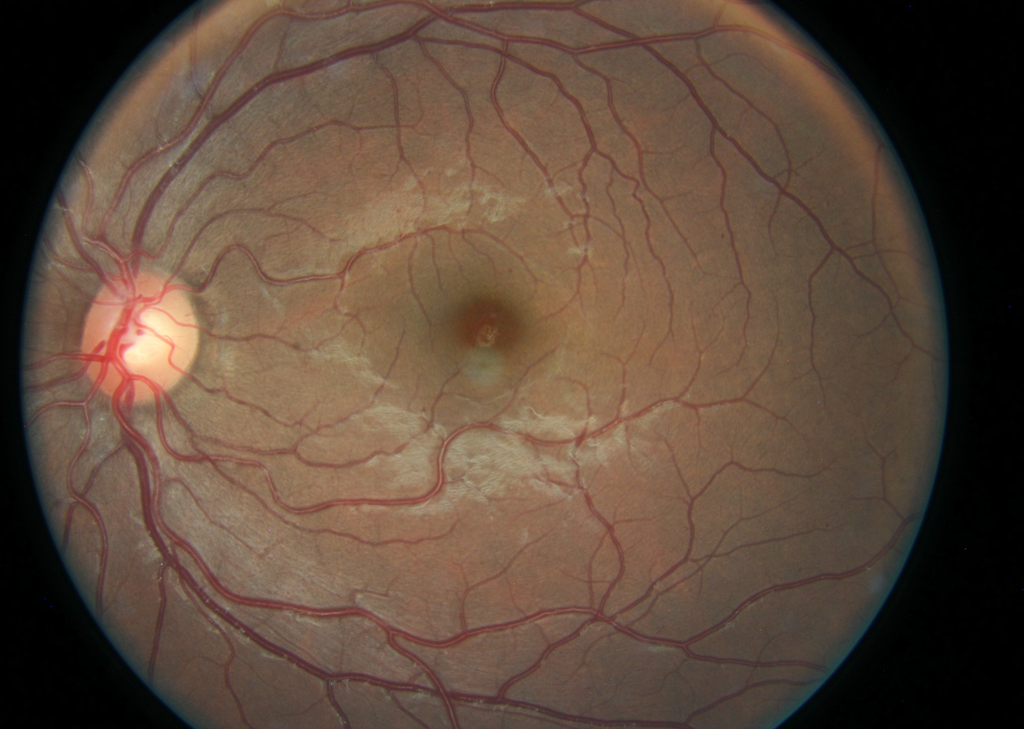
\includegraphics[width=0.43\textwidth]{eyepacs_example}
     \caption*{Eyepacs example}
   \end{figure}
\end{frame}

\begin{frame}{Evaluation}
  Normally: Compare pixel-wise reconstruction error

  \textbf{Difficult} in our case

  Perceptual \textit{\&} adversarial loss improve perceived quality but increase error!

  Rather compare effectiveness as a pre-processing tool
\begin{columns}
  \begin{column}{0.33\linewidth}
    \begin{figure}[h]
      \centering
        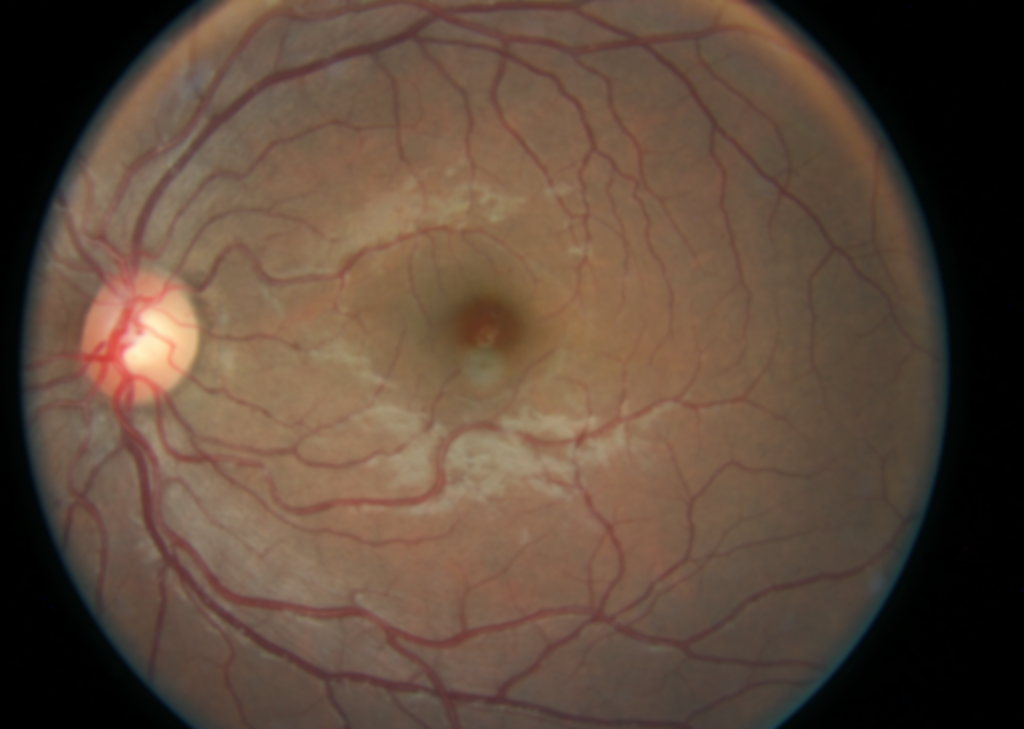
\includegraphics[width=0.9\textwidth]{eyepacs_example_blur}
      \caption*{Blurred}
    \end{figure}
  \end{column}
  \begin{column}{0.33\linewidth}
    \begin{figure}[h]
      \centering
        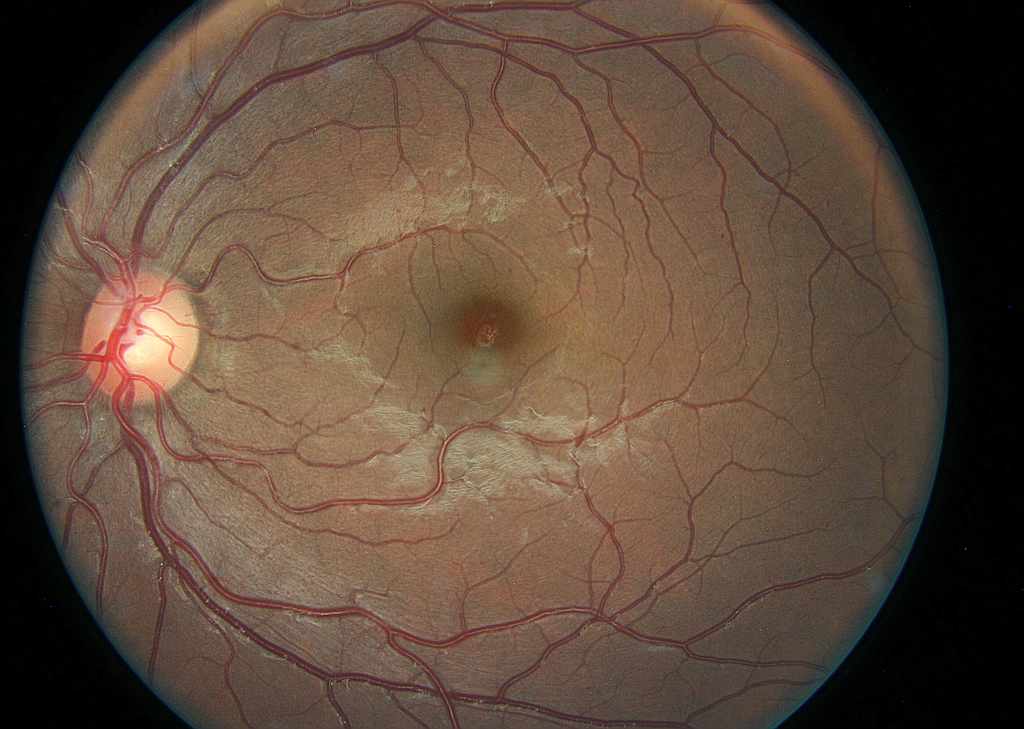
\includegraphics[width=0.9\textwidth]{eyepacs_example_sharp}
      \caption*{Sharpened}
    \end{figure}
  \end{column}  \begin{column}{0.33\linewidth}
    \begin{figure}[h]
      \centering
        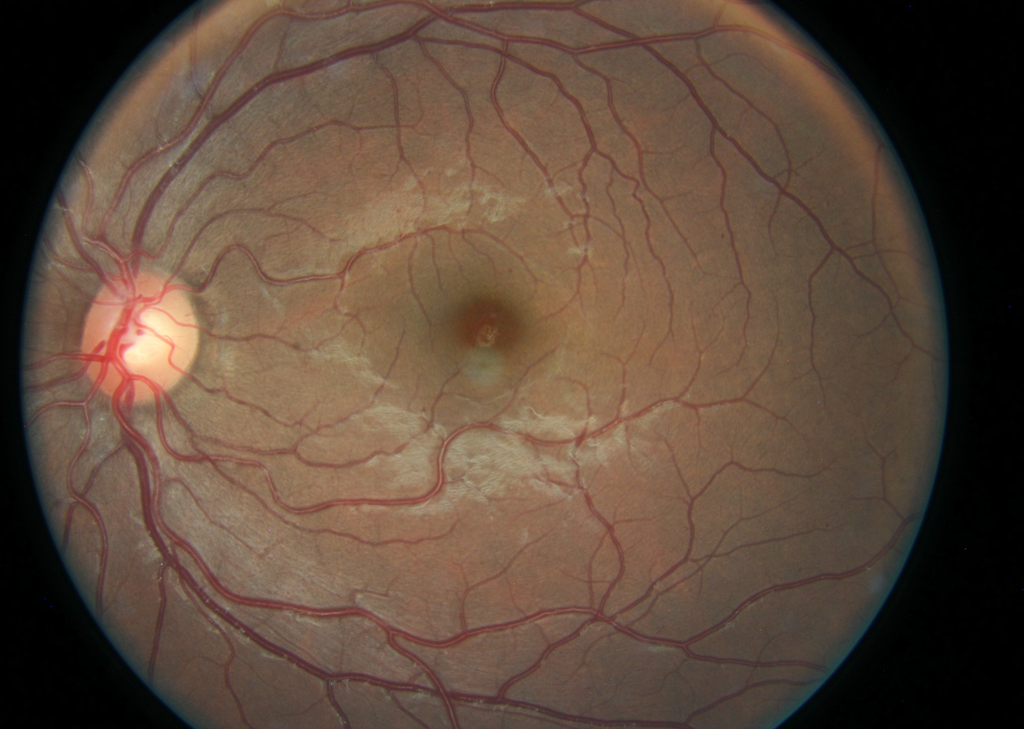
\includegraphics[width=0.9\textwidth]{eyepacs_example}
      \caption*{Ground truth\footnotemark}
    \end{figure}
  \end{column}
  \footnotetext{\url{https://www.kaggle.com/c/diabetic-retinopathy-detection}}
\end{columns}
\end{frame}

\begin{frame} \frametitle{Timeline}
 \begin{figure}[ftbp]
  \centering
  \begin{ganttchart}[
    time slot format=isodate,
    x unit=0.40mm,
    today=2018-01-19,
    y unit chart=5mm,
    ]{2017-10-01}{2018-04-14}
\gantttitlecalendar{year, month} \\
\ganttbar{Data pre-processing}{2017-11-01}{2018-01-15}\\
\ganttbar{Final Evaluation}{2018-03-10}{2018-04-01}\\
\ganttgroup{Implementation}{2017-11-01}{2018-03-10}\\
\ganttbar{$L_1$-based Network}{2017-11-01}{2017-12-30}\\
\ganttbar{Perceptual Loss}{2017-12-15}{2018-01-30}\\
\ganttbar{Adversarial Loss}{2018-01-30}{2018-02-20}\\
\ganttbar{Network Modifications}{2018-02-20}{2018-03-15}
\end{ganttchart}
\end{figure} 

\end{frame}
  
\begin{frame}{Summary}
\begin{itemize}
  \item Real-time super-resolution is realistic
  \item Selection of loss function is important
  \item Need for careful evaluation
\end{itemize}
\begin{figure}[h]
  \centering
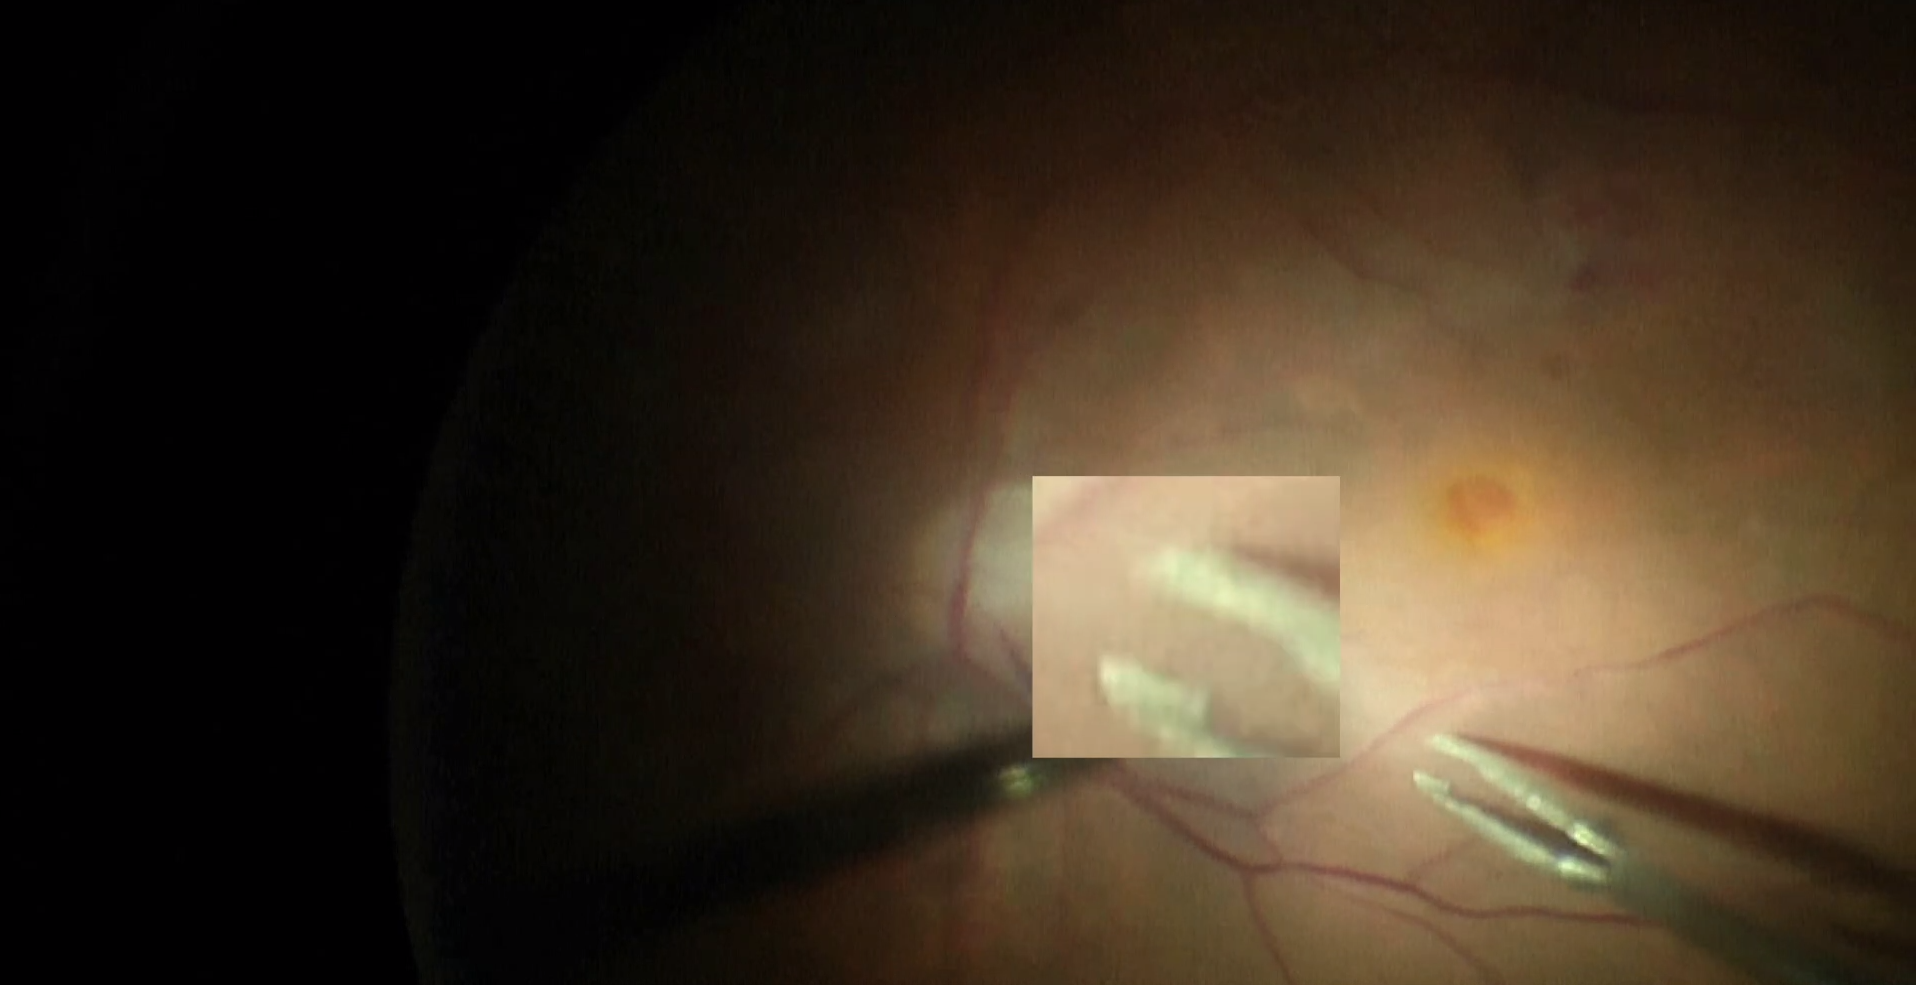
\includegraphics[width=0.9\textwidth]{digitalwindow_screen}
  \caption*{Use case: Digital Window}
\end{figure}
\end{frame}

\end{document}